\chapter{General Parallel Metropolis Hastings}

\section{Introduction of the Algorithm}
The general parallel Metropolis-Hastings algorithm is an algorithm that is based on the fundamental Metropolis-Hastings algorithm with some more parallel modifications. Instead of using different chains to make the algorithm run parallel, the general parallel Metropolis-Hastings algorithm applies a different idea: it generates multiple samples instead of one single sample in each iteration. This idea of parallel execution is inspired to avoid sequential generation of data,\cite{gpmh_broshure} which means that instead of accepting or denying the generated sample, a different way to determine the acceptance of the generated sample points needs to be come up. Since the last sample before the generated sample is carried on if the newly generated sample is denied, we also take the last generated sample into account when designing the general parallel Metropolis Hastings. However, since an array of points is generated, we will randomly select one of the samples as the starting point for the next round of generation.\cite{gpmh_derivation} Suppose that we draw $m$ samples in each iteration, we then have to use $m + 1$ samples to perform the acceptance or rejection. What we then do is to sample $n$ points from these $m$ samples randomly. We construct a probability space by calculating the likelihood for each sample point and sample a subset of these points as the points that should be added to the results.

A detailed explanation of the calculation of acceptance probability is inspired by the derivation from the GMH library of the MUQ framework.\footnote{https://bitbucket.org/mituq/muq2/src/d99f6124bf142922d7973cc60c25d7a518084d12/modules/SamplingAlgorithms/src/GMHKernel.cpp?at=master#GMHKernel.cpp-1,16,45,50,56,58,84} The first step is to construct the acceptance matrix. This matrix has the dimension of  The acceptance probability matrix \( A \) is calculated as follows:

\begin{equation}
A_{ij} = 
\begin{cases} 
\min\left(1, \frac{\exp(r_j - r_i)}{m + 1}\right) & \text{if } i \neq j \text{ and } \text{proposed state } j \text{ is not None} \\
1-\sum_{k \neq i} A_{ik} & \text{if } i = j
\end{cases}
\end{equation}

where $r_j$ is the log density of the $j$th proposed state.

We then calculate the stationary acceptance distribution. It is denoted as $\pi$, which is a vector with a length of $m+1$. To calculate this, we construct the matrix $M = A^T - I$, on which an extra row of 1 is added at the very bottom that represents the weight of the last generated sample. To calculate the stationary distribution, we create the $b$ vector with $0$ everywhere except for the last position, in which a $1$ is set for the same reason mentioned above.\cite{gpmh_derivation} The calculation is then listed as follows:
\begin{equation}
M\pi = b
\end{equation}

After acquiring the acceptance rate vector, we construct a probability space using it, in which we calculate the sum of the vector and then normalize it. Using this vector, we generate $n$ samples from it, including the sample that was generated before. We iterate this process for a certain amount of time and receive the result. To sum up the entire process, we use pseudo-code to illustrate it.
\\


\begin{algorithm}[H]
\SetKwFunction{GeneralParallelMetropolisHastings}{GPMH}
\SetKwProg{Fn}{Function}{:}{}
\KwIn{\tabto{2cm}proposal distribution function, sampling kernel function, likelihood kernel function, initial state, number of iterations, acceptance\_rate\_calculation, num\_proposals, num\_accepted}
\KwOut{\tabto{2cm} list of sampled data points}
\BlankLine

\Fn{\GeneralParallelMetropolisHastings{proposal\_dist, sampl\_kernel, likel\_kernel, init\_state, iterations, acceptance\_rate\_calculation, num\_proposals, num\_accepted}}{
    \tcp{Initialize the samples list with the initial state}
    samples $\leftarrow$ [init\_state]
    old $\leftarrow$ init\_state
    
    \For{i $\leftarrow$ 1 \KwTo iterations}{
        \tcp{Generate a new sample from the sampling kernel}
        generated\_samples $\leftarrow$ [old] \\

        \For{j $\leftarrow$ 1 \KwTo num\_proposals}{
            generated\_samples.append(sampl\_kernel(old))\\
        }
        
        \tcp{Calculate the acceptance probability}
        acceptance\_rates = acceptance\_rate\_calculation(generated_samples)
        
        \tcp{Decide to accept or reject the new sample}
        \tcp{random\_sampling is a function that takes two parameters, sampling randomly the number of times given in the first parameter from the array given in the second parameter using the acceptance rate provided in the third parameter}
        res $\leftarrow$ random\_sampling(num\_accepted, num\_proposed, acceptance\_rates)
        samples.append(res)
        old = random(res)
    }
    \Return samples
}

\caption{General Parallel Metropolis-Hastings Algorithm}
\end{algorithm}


\section{Evaluation}
After discussing the algorithm itself, we run the algorithm and generate data that can be used to analyze. In this section, we will first try to observe the algorithm regarding the number of samples generated and accepted in each iteration through ratio and amount tests. Afterward, further investigation regarding input parameters is conducted.

\subsection{Ratio Test}
The very first test for evaluation is called the ratio test. In this test, we investigate the ratio between the numbers generated and the numbers accepted. This test is conducted for us to find the most optimal ratio of both parameters for the Bayesian inference problem. We fix the number of accepted samples being five, while the number of generated samples is a variable. The tested scenarios include 5 generated samples for a ratio of 1, 10 generated samples for a ratio of 2, 20 generated samples for a ratio of 4, 40 generated samples for a ratio of 8, and 80 generated samples for a ratio of 10. As we can see from figure 6.1, the accuracy of the Bayesian inference goes up as the ratio of the generated sample amount against the accepted sample amount goes up. The larger the ratio is, the more accurate the Bayesian inference would be. However, the trade-off would be the run time, as the run time grows. There is an obvious exponential relationship between the run time and the ratio. Therefore, we need to consider the trade-off between accuracy and efficiency while selecting an appropriate ratio.

\begin{figure}[H]
    \centering
    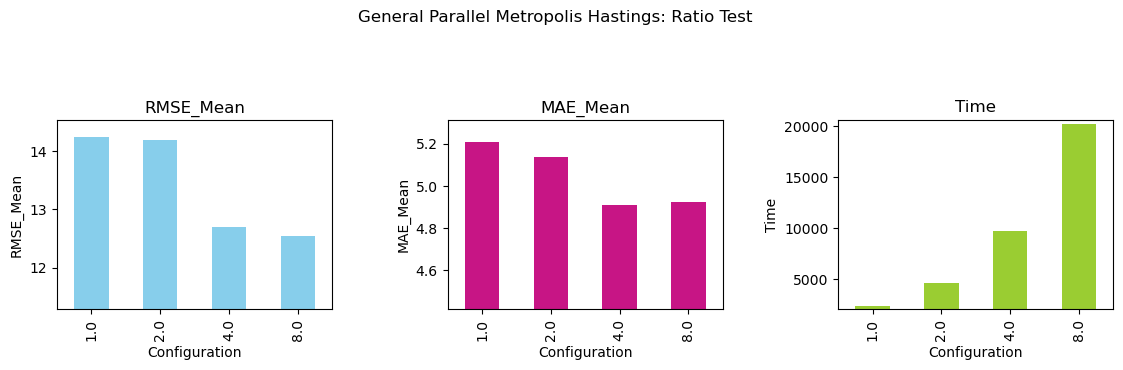
\includegraphics[width=1\textwidth]{figures/gpmh/ratio_test.png}
    \captionsetup{width=.8\textwidth}
    \caption{Comparison of the accuracy and the efficiency of general parallel Metropolis Hastings algorithms based on the ratio between numbers generated and accepted for each iteration}
    \label{fig:enter-label}
\end{figure}

\subsection{Amount Test}
We move on to the amount test, in which we investigate the optimal amount of samples that need to be generated for each iteration. We fix the ratio between the generated samples and the accepted samples being $2$. The tested scenarios include 10 generated samples with 5 being accepted, 20 generated samples with 10 being accepted, 40 generated samples with 20 being accepted, 80 generated samples with 40 being accepted, and 100 generated samples with 50 being accepted. In comparison with the ratio test, the differences are not that obvious in this case. For the RMSE, better performances of the Bayesian inference are delivered for higher amounts, whereas the MAE data do not differ too much from each other. For efficiency, faster execution happens also in higher ranges of amount numbers. Therefore, the more samples generated in each iteration, the faster and more accurate the algorithm will be.

\begin{figure}[H]
    \centering
    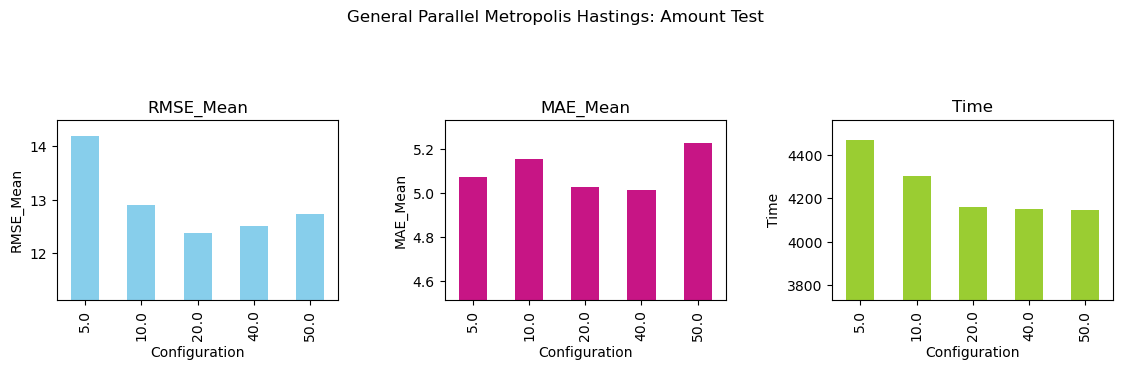
\includegraphics[width=1\textwidth]{figures/gpmh/amount_test.png}
    \captionsetup{width=.8\textwidth}
    \caption{Comparison of the accuracy and the efficiency of general parallel Metropolis Hastings algorithms based on the amount of technique of handling samples generated out of bounds}
    \label{fig:enter-label}
\end{figure}

\subsection{Sampling out of bounds}
After investigating the relationship between generated sample numbers and the accuracy and efficiency metrics, we now switch gears to the input parameters. For the first input parameter, we take a look at the sampling out-of-bounds methods. As it was mentioned before, we apply three methods when handling samples that are generated out of bounds: ignoring, reflecting boundary, and aggregation. These three methods are also used in the general parallel Metropolis-Hastings algorithm. The benchmark result is shown in Figure 6.3. Unlike the case in the fundamental implementation, all three variants show little difference from each other in terms of accuracy. In terms of efficiency, the ignoring method still outperforms the other two methods just like the case for the fundamental implementation, however not by a lot. The selection of the method usage is therefore not the most relevant selection for the general parallel Metropolis Hastings algorithm considering the minimal impact on the accuracy and efficiency metrics.

\begin{figure}[H]
    \centering
    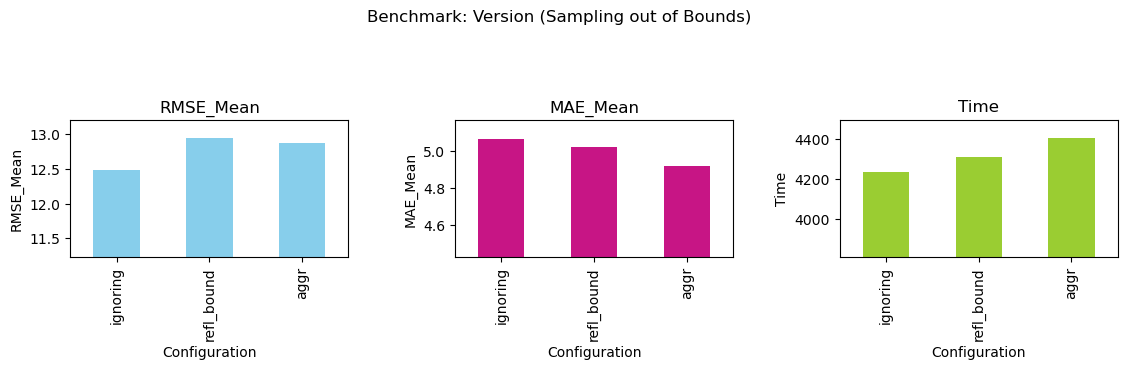
\includegraphics[width=1\textwidth]{figures/gpmh/sotb.png}
    \captionsetup{width=.8\textwidth}
    \caption{Comparison of the accuracy and the efficiency of general parallel Metropolis Hastings algorithms based on the dependent likelihood function standard deviation}
    \label{fig:enter-label}
\end{figure}

\subsection{Initial States}
Another input parameter that might impact the resulting outcome is the initial states. The selection of the initial state does not result in a drastic difference in the accuracy metrics for the fundamental Metropolis-Hastings, and this is exactly the case here. For both metrics, the value for each input option of initial states does not vary much from each other. For efficiency, on the other hand, the initial state had a drastic influence on the run time. The fundamental algorithm with the best initial state could achieve less than twice the time that with the worst initial state. This is the complete opposite of the general parallel Metropolis-Hastings algorithm, in which algorithms with all different selections of initial states deliver similar results, all with a run time of around 4000 seconds. This means that the selection of the initial state does not have a big influence on the overall result of the general parallel Metropolis-Hastings algorithm. 

\begin{figure}[H]
    \centering
    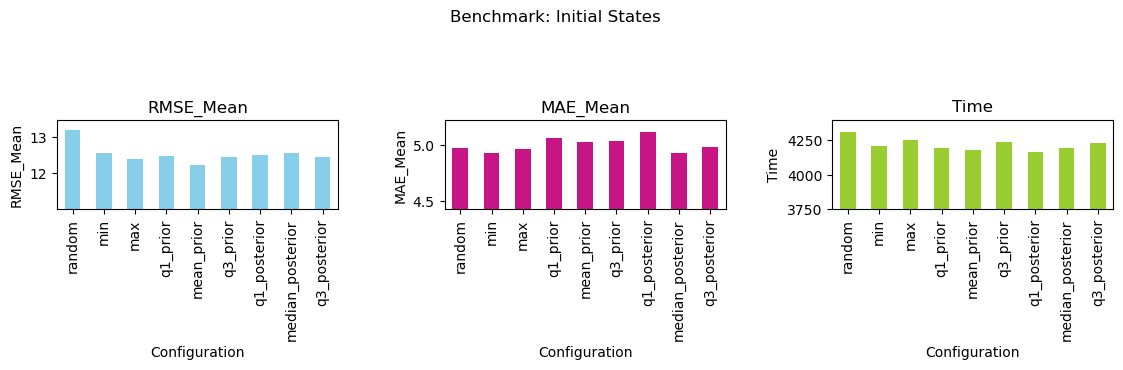
\includegraphics[width=1\textwidth]{figures/gpmh/init_states.png}
    \captionsetup{width=.8\textwidth}
    \caption{Comparison of the accuracy and the efficiency of general parallel Metropolis Hastings algorithms based on the selection of initial states}
    \label{fig:enter-label}
\end{figure}

\subsection{Dependent Likelihood Kernel Factor}
The behavior of the dependent likelihood kernel factor for the general parallel Metropolis-Hastings algorithm is far different from the one for the fundamental Metropolis-Hastings algorithm. For the case here, the accuracy shows a certain level of irregularity, with the value $0.6$ delivering the most optimal result. For efficiency, on the other hand, every run using different input values results in almost the same run time, except $0.8$ as an anomaly, requiring more time than any other input values. Therefore, the value $0.6$ is the most optimal choice for this case here.

\begin{figure}[H]
    \centering
    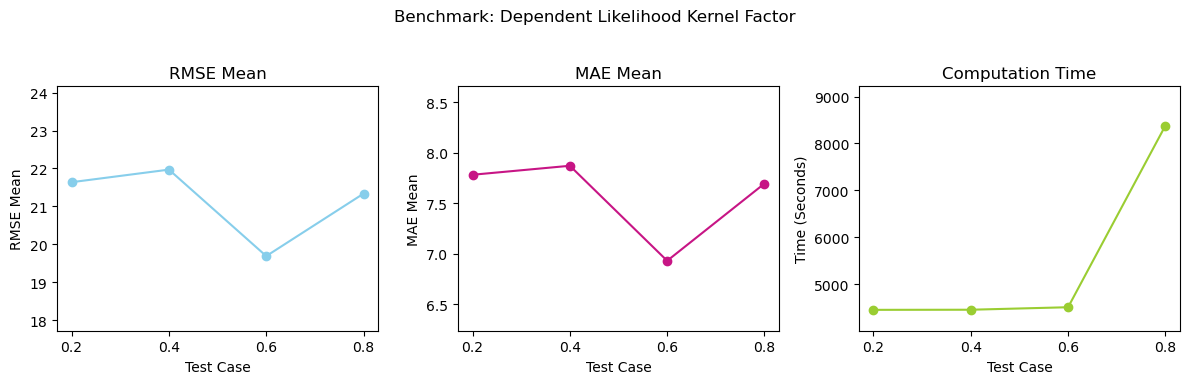
\includegraphics[width=1\textwidth]{figures/gpmh/dependent_likelihood_kernel_factor.png}
    \captionsetup{width=.8\textwidth}
    \caption{Comparison of the accuracy and the efficiency of general parallel Metropolis Hastings algorithms based on the dependent likelihood function standard deviation}
    \label{fig:enter-label}
\end{figure}


\subsection{The Rest of Input Parameters}
For the rest of the input parameters, detailed explanations are spared for this chapter, since they have similar results as the fundamental Metropolis-Hastings algorithm. These are listed here as follows: 
\begin{itemize}
    \item Transition kernel factor: Not many differences in terms of accuracy. For the efficiency part, the run time of the algorithm does not matter from each other too much, apart from an anomaly point at the very last, which has also occurred in the fundamental Metropolis Hastings algorithm.
    \item Independent likelihood kernel factor: there is a peak on which the accuracy performance is the worst, $3$ in the case of general parallel Metropolis Hastings. Centered from this peak, the result gradually becomes more accurate. The run time for each run does not differ from each other by much.
    \item Dependent likelihood kernel factor: No big differences of accuracy across different input values. For the run time, both extreme input values ($0.2$, $0.8$) provide the best performances, while the overall differences between the performances are not significant.
    \item Burn in: No big differences of both metrics across different input values.
    \item Effective Sample Size: No big differences of both metrics across different input values.
\end{itemize}

\section{Comparison of General Parallel Metropolis Hastings with the Fundamental Implementation}
After performing an analysis of the general parallel Metropolis-Hastings algorithm, a comparison of it and the fundamental Metropolis-Hastings algorithm is made here. For most cases, the RMSE score of the algorithm is around $12$ and the MAE score is around $5$. This improves significantly from the fundamental Metropolis-Hastings algorithm, which delivers an RMSE score of around $20$ and an MAE score of around $9$. However, the fastest run of the fundamental Metropolis-Hastings algorithm is around $1400$ seconds in comparison to around $4000$ seconds of the general parallel Metropolis-Hastings algorithm. Between better efficiency and better accuracy, there is a trade-off that needs to be considered.